\documentclass{article}

\usepackage[utf8]{inputenc}
\usepackage{amsmath, enumitem, url}
\usepackage{xcolor}
\usepackage[margin=1in]{geometry}

% For figures.
% Package float, adds the H option which forces figure placement.
% \usepackage[demo]{graphicx}
\usepackage{graphicx, float, subfig}
\graphicspath{ {./figures/} }

\newcommand\todo{\textcolor{red}{\textbf{[TODO:] }}}

\title{Learning end-to-end control for duckiebot driving}
\author{Group: Dropouts}
\date{June 2021}

\begin{document}
\maketitle

\section{Group Information}

Members:
\begin{itemize}
    \item Keyan Pishdadian (keyanp@cs.washington.edu)
    \item Jakub Filipek (balbok@cs.washington.edu)
    \item Kyle Deeds (kdeeds@cs.washington.edu)
\end{itemize}

\noindent Source code for behavior cloning approach:
\newline
\url{https://github.com/keyan/duckiebot_behavior_cloning}

\noindent Source code for reinforcement learning approach:
\newline
\url{https://github.com/balbok0/cse571-sp21-project-2-dropouts}

\section{Task Overview}

In this project we sought to explore methods for learning an end-to-end control policy that would allow the duckiebot to navigate tracks autonomously. Our goal was to enable the duckiebot and have it navigate around an entire track without any major driving infractions (defined as exiting the lane or going off the road), using only monocular camera data. Ideally this system would be robust enough to generalize to new tracks and work on the real robot as well as in simulation.

Inspired by previous efforts in learning end-to-end control for driving using deep reinforcement learning \cite{DBLP:journals/corr/abs-1807-00412} our original plan was to evaluate a selection of reinforcement learning algorithms to solve this task. Knowing that reproducing reinforcement results is difficult and often unsuccessful \cite{henderson2019deep}, we planned to also experiment with a behavior cloning approach inspired by prior work from NVIDIA where a convolutional neural network was trained to steer a car using only image data \cite{DBLP:journals/corr/BojarskiTDFFGJM16}.

\section{Environment Setup}

We performed experimentation and evaluation of our agents in simulation and on the real robot primarily relying on the ``AI Driving Olympics" infrastructure \cite{zilly2019ai}. Our agent was structured into the AIDO submission format and then executed either in simulation or on the real duckiebot. We used the default episode length configuration, which runs agents for 60 seconds. The AIDO submission format requires structuring an agent that obeys the AIDO agent interface and accepts image observations and outputs control commands. We referenced the baseline implementations for both reinforcement learning and behavior cloning submission types, \url{https://github.com/duckietown/challenge-aido_LF-baseline-RL-sim-pytorch} and \url{https://github.com/duckietown/challenge-aido_LF-baseline-behavior-cloning}, respectively.

\subsection{Simulation}

We used the \texttt{gym-duckietown} simulator \cite{gym_duckietown} for training and evaluation of agents when using a reinforcement learning approach, as well as for evaluation when using behavior cloning (through the AIDO submission infrastructure). For reinforcement learning we only ran evaluation on the most simple map type, ``loop\_empty", which is an square map with no obstacles. Evaluations for behavior cloning used a specific ``challenge", \texttt{aido-LF-sim-validation} which runs the agent on a static selection of maps and ranks submissions against other users.

\subsection{Real World}

Evaluation on the real duckiebot was done on four different maps (\ref{fig:maps}), with a 60 second maximum episode duration. Only map2 was used for real robot data collection.

\begin{figure}[H]
\centering
    \subfloat[\centering map1]{{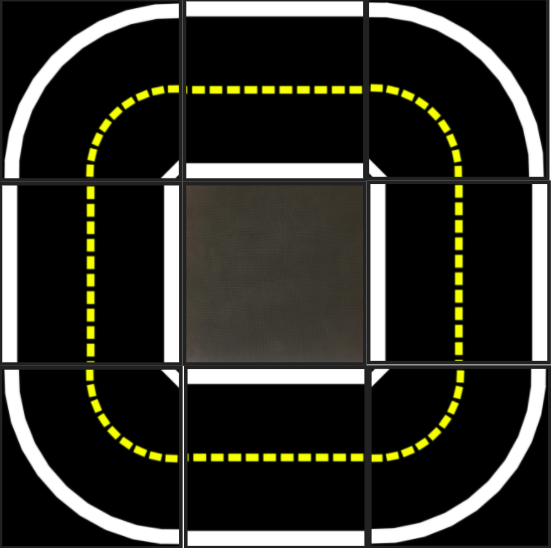
\includegraphics[width=5cm]{map1} }}
    \qquad
    \subfloat[\centering map2]{{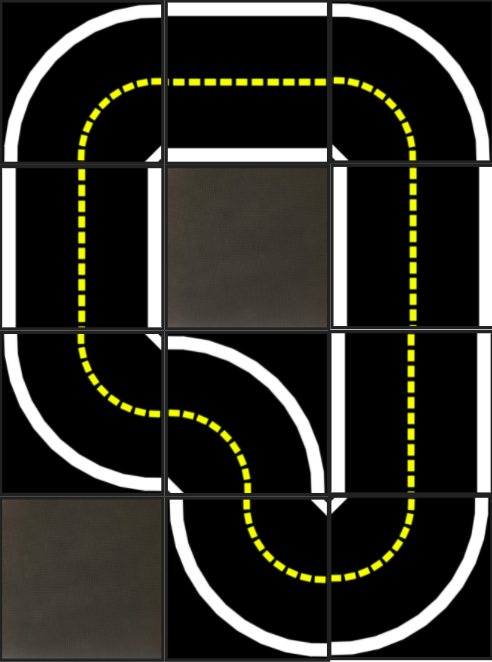
\includegraphics[width=5cm]{map2} }}
    \qquad
    \subfloat[\centering map3]{{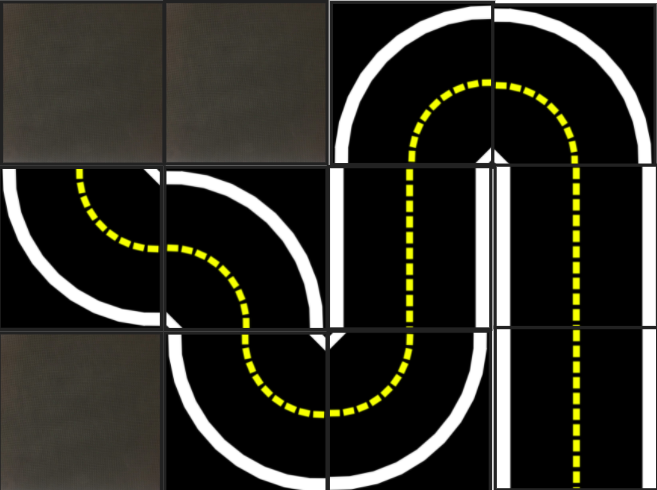
\includegraphics[width=5cm]{map3} }}
    \qquad
    \subfloat[\centering map4]{{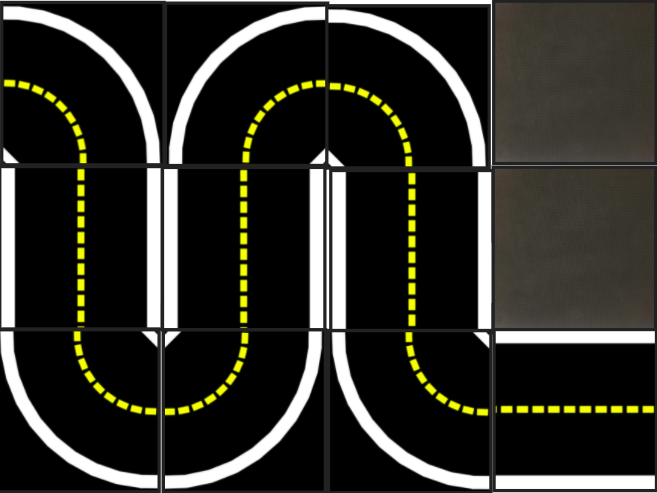
\includegraphics[width=5cm]{map4} }}
    \caption{Digital overview of the four maps used for real-world evaluation.}
    \label{fig:maps}
\end{figure}

\begin{figure}[H]
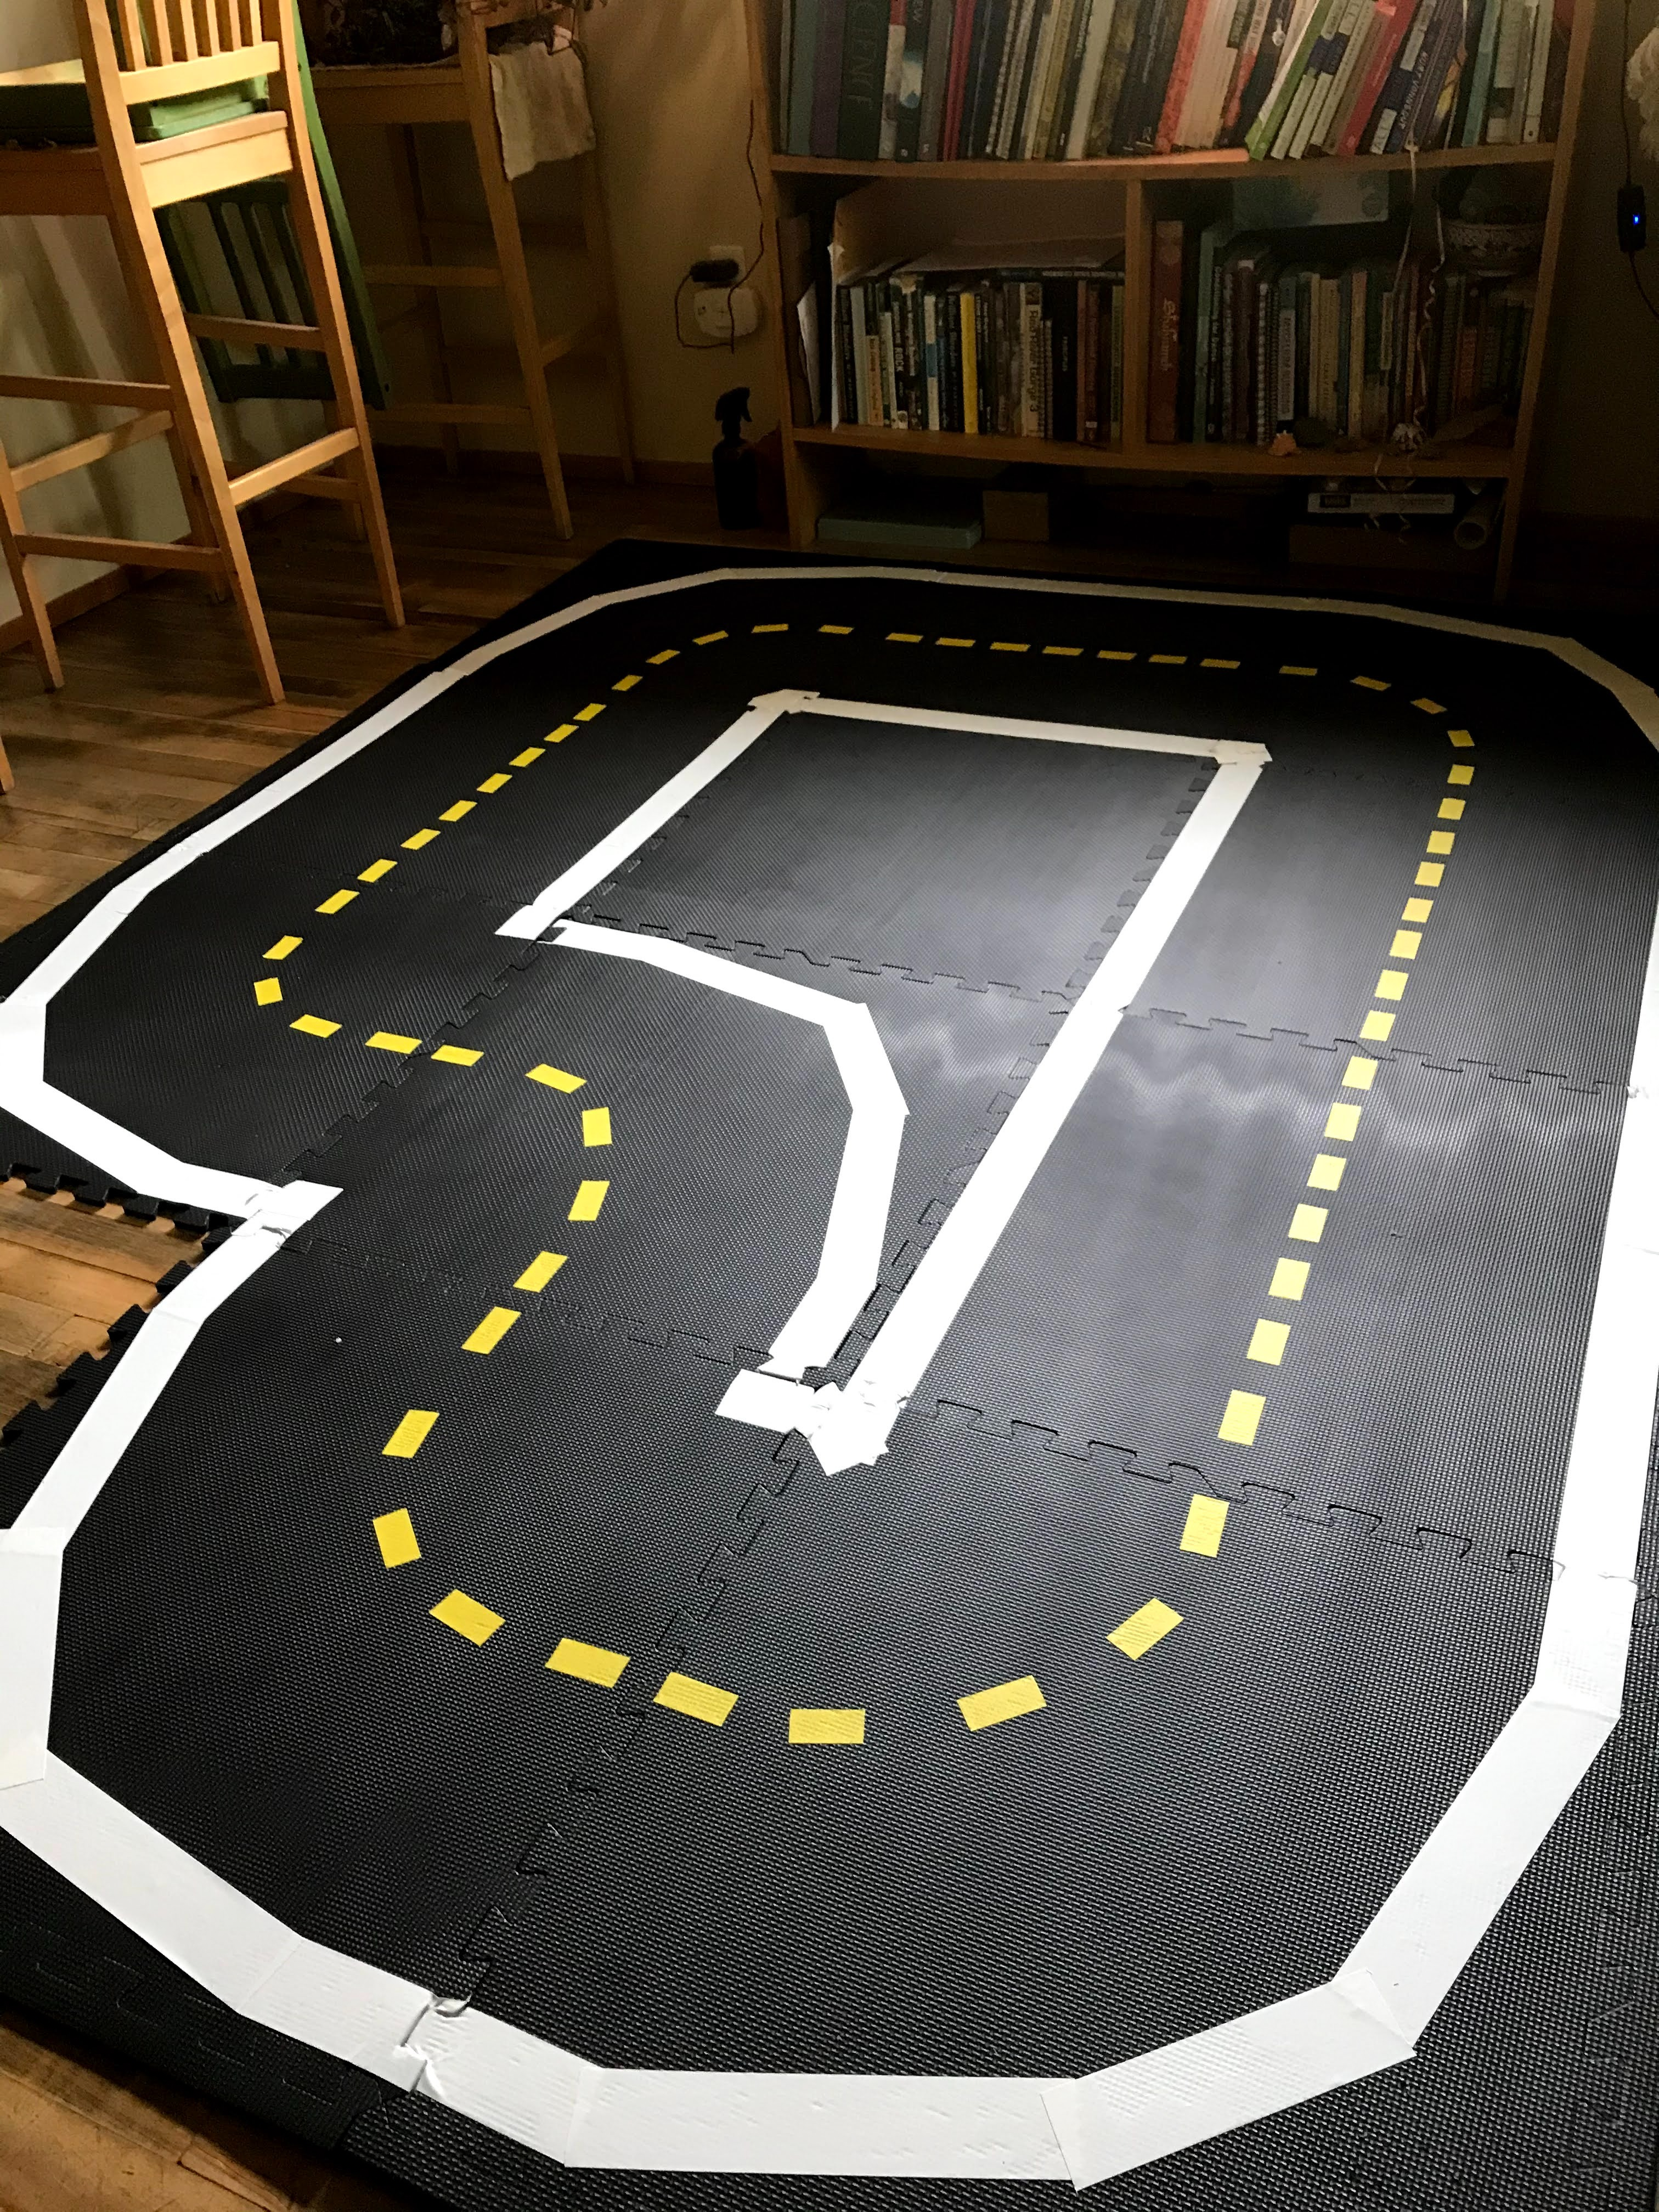
\includegraphics[angle=-90,width=8cm,keepaspectratio]{map2_real}
\centering
\caption{Photo of physical layout of map2.}
\label{fig:map2_real}
\end{figure}

\section{Reinforcement Learning Approach}

Our initial solution was to use the \texttt{gym-duckietown} environment to train an agent using a model-free off-policy Q-learning algorithm, for which we explored both DQN \cite{DBLP:journals/corr/MnihKSGAWR13} and DDPG \cite{journals/corr/LillicrapHPHETS15} algorithms. Our training code leveraged pre-written implementations of both algorithms provided through the RLLib package \cite{DBLP:journals/corr/abs-1712-09381}. We leveraged the existing default reward function provided by the gym environment (\url{https://git.io/JGnsg}) which is a linear function of the robot speed, position within the lane relative to the right line, and proximity to obstacles.

\todo Some brief amount of discussion about DQN and DDPG that shows we at least understand it \\

Unfortunately we were unsuccessful in achieving reasonable training results with this method, with our agent consistently showing an inability to increase average reward obtained despite experimenting with domain randomization in the simulator, training across multiple maps, and performing hyperparameter search (Figure \ref{fig:rl_training}). Our initial impression was that training an agent to perform well in simulation would be straightforward and the main challenge would be in transferring the agent to the real environment. When our agents failed to show any promising results during training and subsequently failed to perform in simulation at all, we decided to abandon this approach. Videos of evaluation of these agents in simulation can be found at \url{https://youtu.be/SDZ59_2zhGg} (DQN agent) and \url{https://youtu.be/1xL8b2MK6N4} (DDPG agent).

\begin{figure}[H]
\centering
    \subfloat{{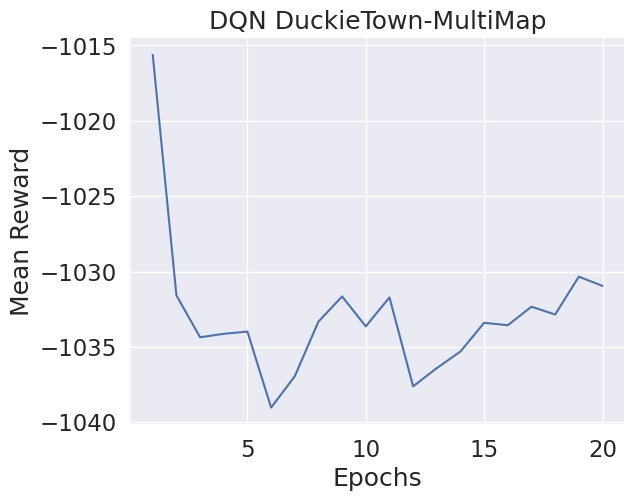
\includegraphics[width=7cm]{dqn_reward} }}
    \qquad
    \subfloat{{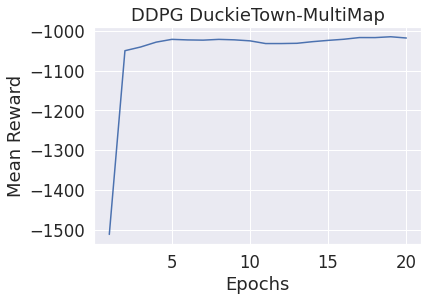
\includegraphics[width=7cm]{ddpg_reward} }}
    \caption{Mean reward obtained per epoch during training of the DQN (a) and DDPG (b) solutions. Both solutions failed to improve mean reward. Here only 20 epochs are shown, but the plateau in reward obtained was observed even when trained for many more epochs.}
    \label{fig:rl_training}
\end{figure}

\section{Behavior Cloning Approach}

Our focus then shifted towards a strategy where we would train a convolutional neural network (CNN) that would accept a single camera image from the robot at each timestep and then output a prediction for the linear and angular velocity that the robot should apply. This approach was influenced by work from NVIDIA where this technique was applied to predicting a single value representing the steering of the vehicle \cite{DBLP:journals/corr/BojarskiTDFFGJM16}. We designed several CNN models (discussed in Section \ref{sec:model_arch}) and trained them on a combination of simulation and real world data, then evaluated these models using the AIDO leaderboard and on the real duckiebot. An high-level overview of this system is shown in Figure \ref{fig:cnn_overview}.

\begin{figure}
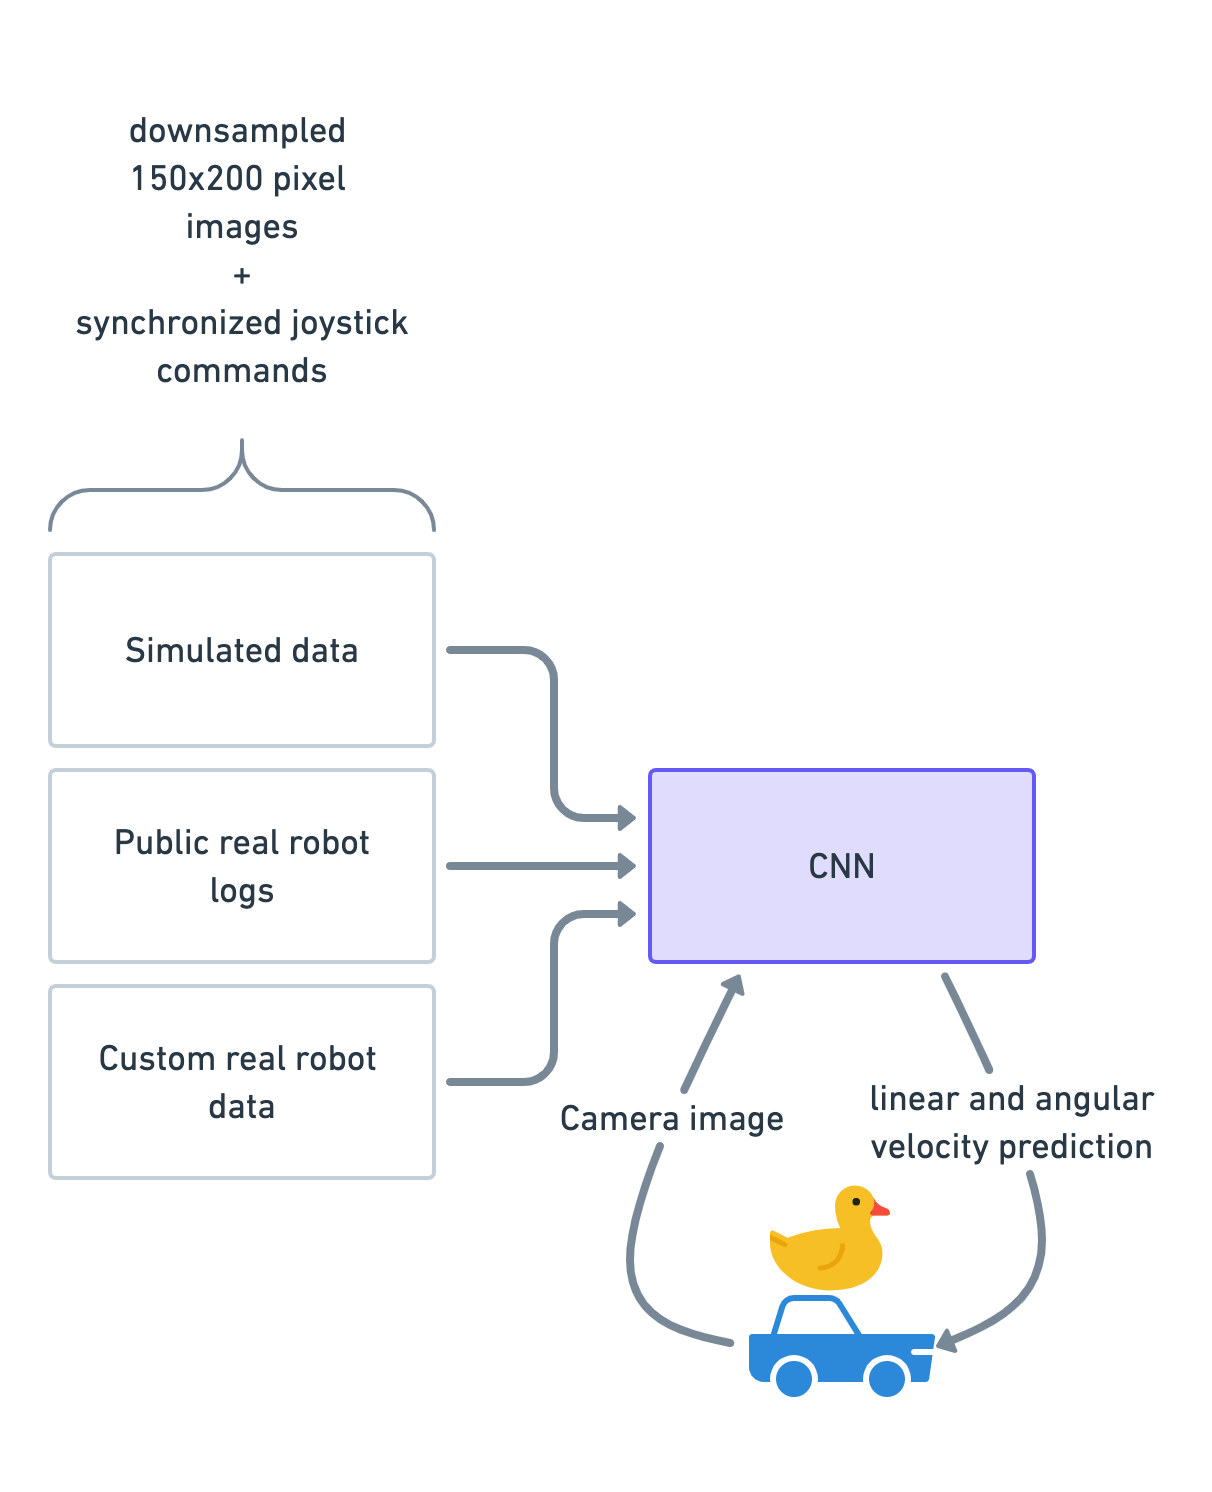
\includegraphics[width=8cm,keepaspectratio]{cnn_overview}
\centering
\caption{Overview of input training data and data flow during inference for the behavior cloning approach to end-to-end control. At runtime the robot passes each observation frame to the CNN model to produce predicted linear and angular velocities. These velocities are converted to left and right wheel velocity commands which are issued to the robot.}
\label{fig:cnn_overview}
\end{figure}

\subsection{Data Preparation}

Data collection from simulation in the \texttt{gym-duckietown} environment is easier, faster, and less noisy than real world data, so the overall data strategy was to focus on collecting a large volume of simulated data and augmenting its applicability to real robot evaluation by including a smaller amount of real robot data extracted from ROS bags.

To collect simulated data, a built-in demo was executed in the simulator that uses a pure pursuit controller \cite{DBLP:journals/corr/PadenCYYF16} to geometrically determine the optimal robot controls, the resulting image observations and joystick controls were aggregated. Image observations from simulation were downsampled to 150x200 and domain randomization was applied during the simulation runs to help prevent overfitting to the simulation environment.

Real robot data was collected through a combination of accessing publicly available ROS bags \cite{paull17duckietown} and ROS bags recorded from demonstrations with one of our own robots on map2 (Figure \ref{fig:maps}b). When selecting public robot logs, we attempted to find executions which were successfully navigating the map, were free of obstacles, and contained turns. For the custom data robot controls were given by a human driver.

% \begin{figure}[H]
\begin{figure}
\centering
    \subfloat[\centering Simulated data]{{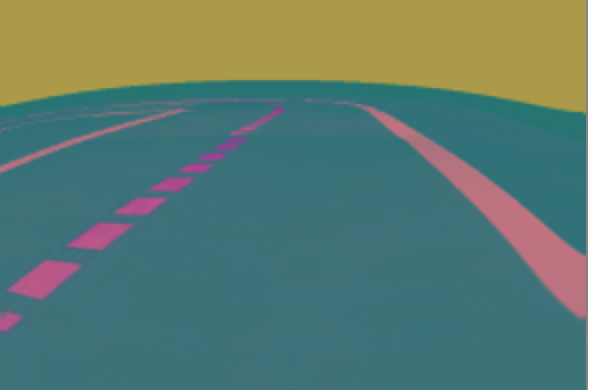
\includegraphics[width=4cm]{sim_data} }}
    \qquad
    \subfloat[\centering Public log data]{{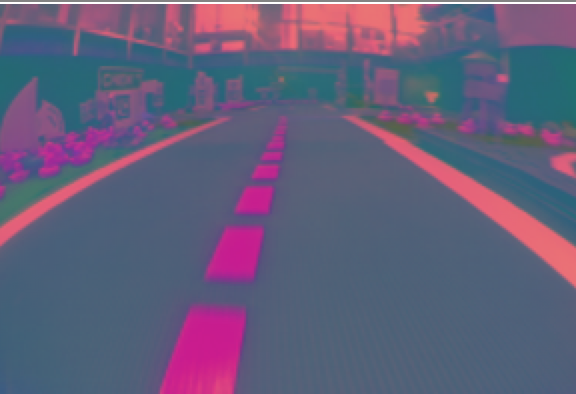
\includegraphics[width=4cm]{log_data} }}
    \qquad
    \subfloat[\centering Custom data]{{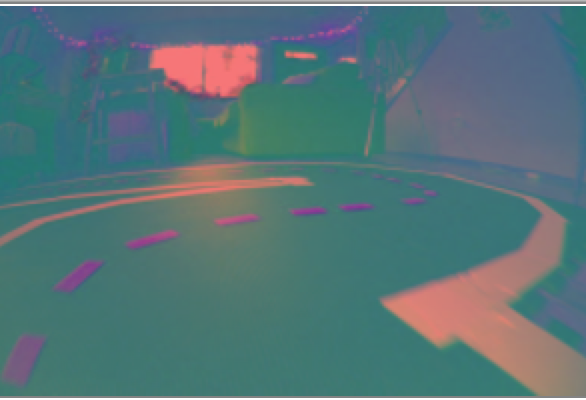
\includegraphics[width=4cm]{custom_data} }}
    \caption{Example frames from the three different data sources used for training. Observations are downsampled 150x200 pixel images.}
    \label{fig:data_examples}
\end{figure}

Ultimately we used two final datatsets. The largest (henceforth ``dataset A") was used for training the initial model and consisted of 58,414 total observation frames with associated controls, this was a mix of simulated data collected from \texttt{gym-duckietown} (50,337 frames) and public real robot data (8,077 frames). The second dataset (henceforth ``dataset B") was used for experimenting with fine tuning our models and consisted of 15,560 total frames, this only contained our custom real robot data.

\subsection{Model Architectures} \label{sec:model_arch}

    Our experiments were focused around two model architectures, the first was an attempt to reproduce results from NVIDIA \cite{DBLP:journals/corr/BojarskiTDFFGJM16} which we named the ``nvidia" model (Figure \ref{fig:model_arch}a). In order to predict two values (linear and angular velocity) two separate instantiations of this model were created with disjoint weights. The only major deviations from the originally published model were the use of leaky rectified linear unit (LeakyReLU) activations and dropout in-between linear layers ($p=0.5$).
    The second architecture used a smaller number of total parameters, shared weights across the convolutional layers, and two outputs preceded by small disjoint linear layers (Figure \ref{fig:model_arch}b). We named the initial version of this model ``modelv0", subsequent experimentation produced a second version ``modelv1" which substituted ReLU activations for LeakyReLU, and added dropout to the final linear layers ($p=0.5$) and the shared convolutional layers ($p=0.1$).

\begin{figure}
    \subfloat[\centering]{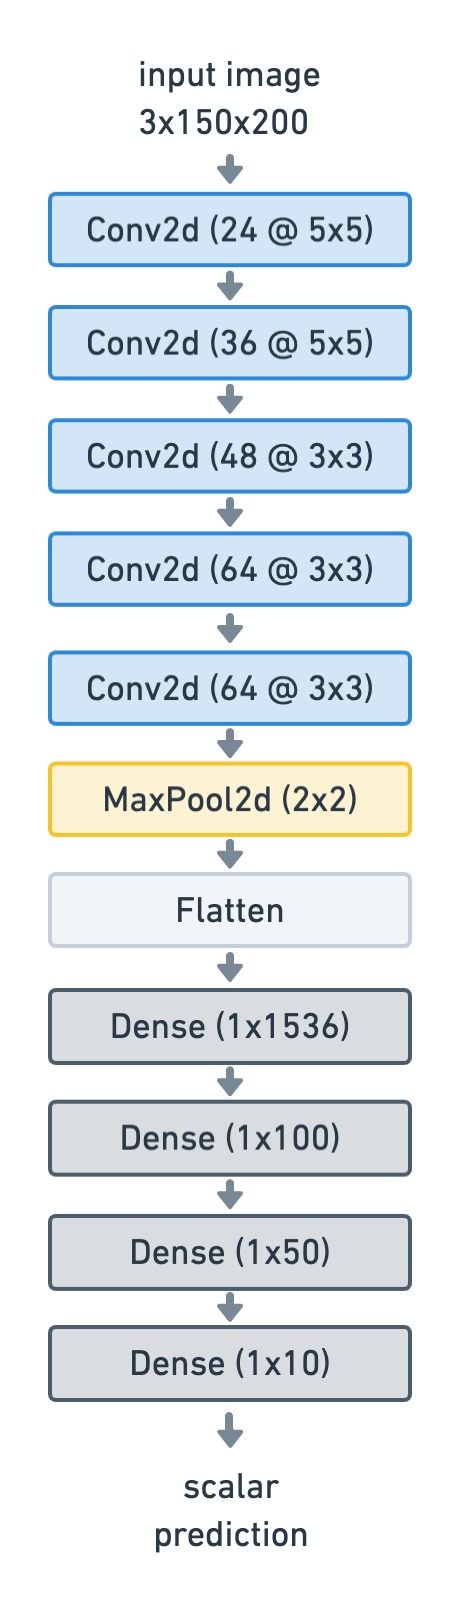
\includegraphics[width=.22\textwidth,keepaspectratio]{nvidia_arch}}
    \subfloat[\centering]{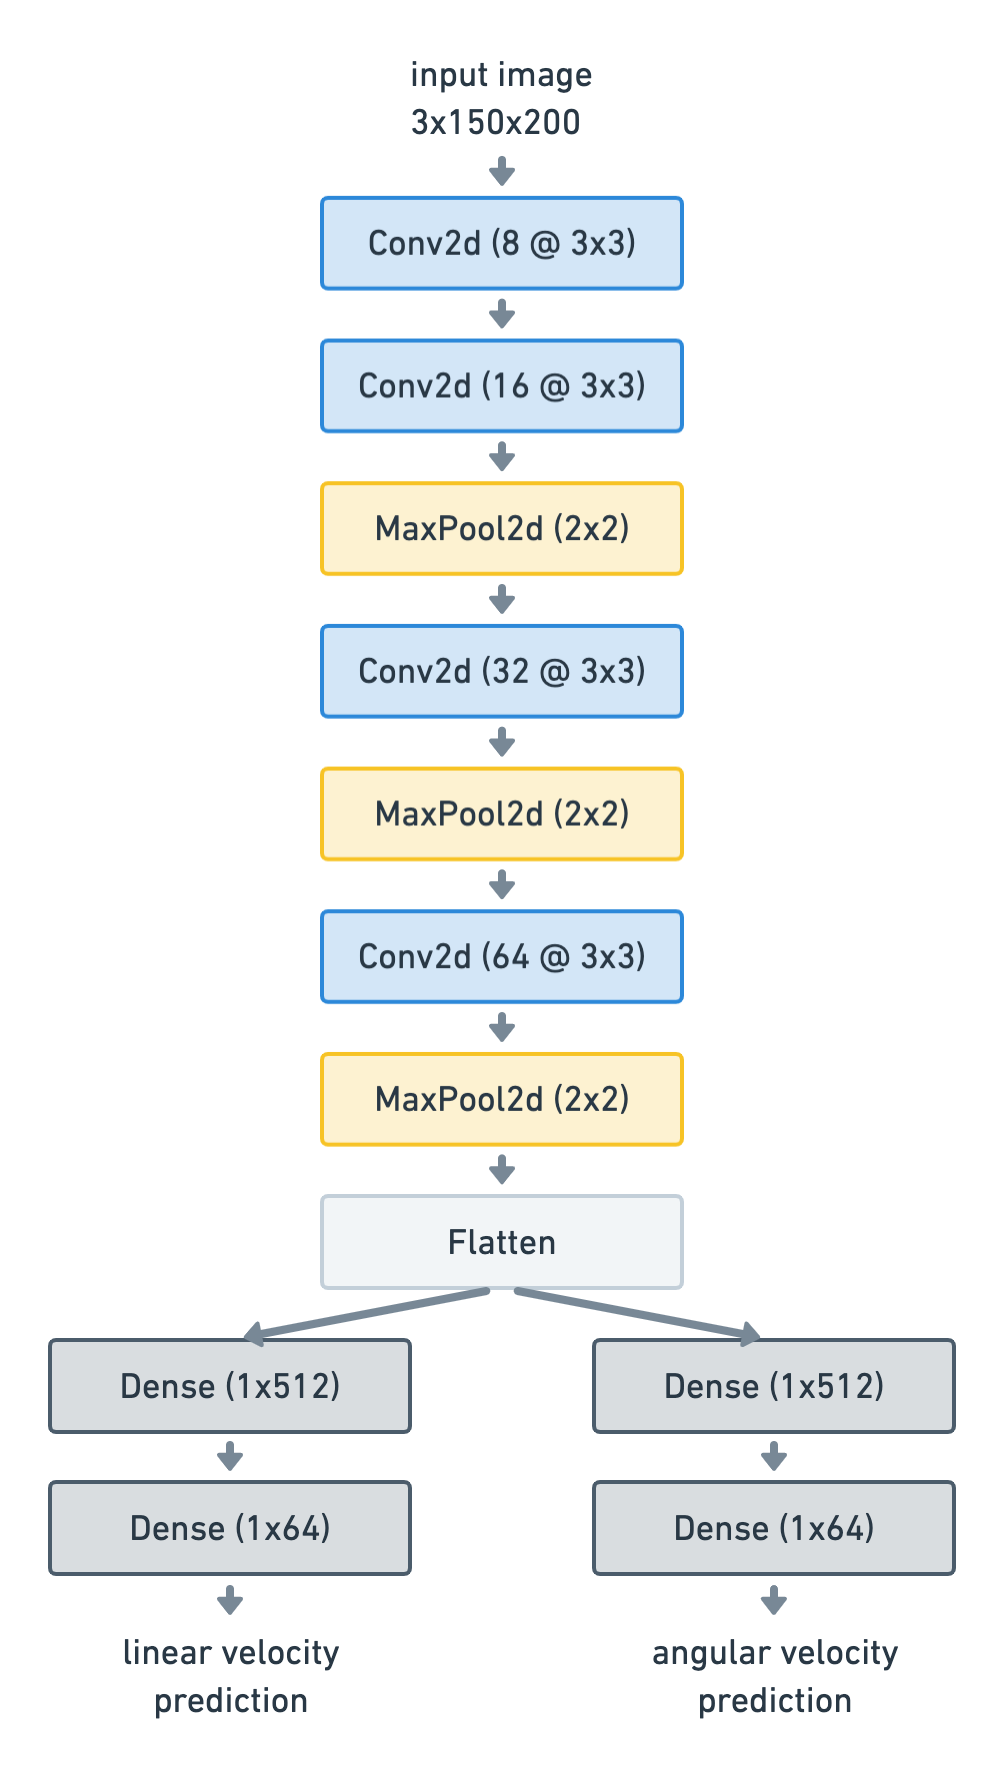
\includegraphics[width=.43\textwidth,keepaspectratio]{dual_cnn_arch}}
\centering
    \caption{Overview of the two primary model architectures evaluated in this work. (a) features a larger number of total parameters and no shared weights, each of the two prediction values retain their own copy of the model (b) uses shared convolutional layers and small linear layers preceding each of the two outputs.}
\label{fig:model_arch}
\end{figure}

\subsection{Training}
All training was done using stochastic gradient descent and mean squared error loss. The models were trained initially on the aggregated dataset (``dataset A") for 200 epochs, results in Figure \ref{fig:training_results}. As the ``nvidia" model did not show promising results during training, it was excluded from further experimentation. Then ``modelv0" and ``modelv1" were fine tuned for 50 epochs using the custom real robot dataset (``dataset B"), results in Figure \ref{fig:fine_tuning_training_results}.

\begin{figure}
  \centering
  \raisebox{35pt}{\parbox[b]{.1\textwidth}{nvidia}}%
  \subfloat{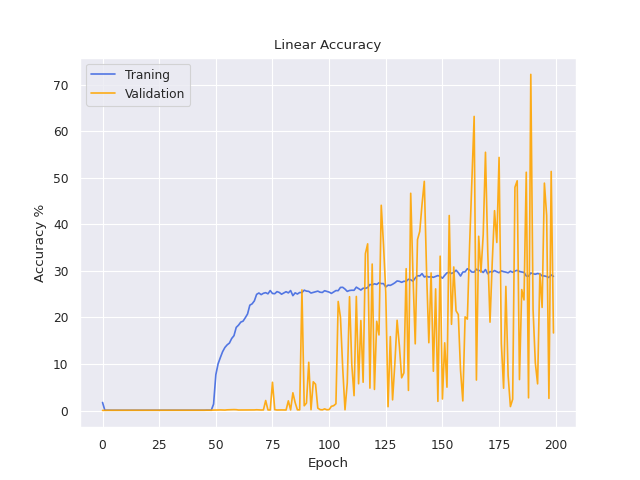
\includegraphics[width=.28\textwidth]{nvidia_linear_accuracy}}\hfill
  \subfloat{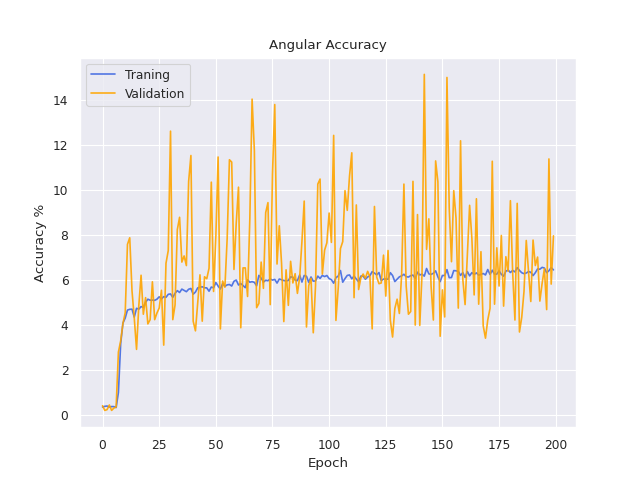
\includegraphics[width=.28\textwidth]{nvidia_angular_accuracy}}\hfill
  \subfloat{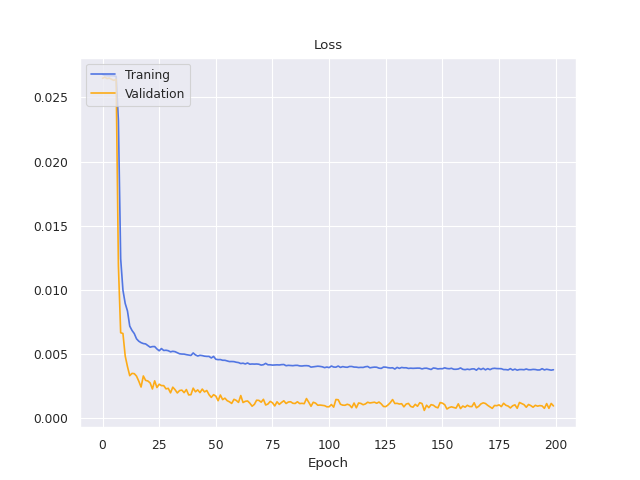
\includegraphics[width=.28\textwidth]{nvidia_loss}}\par
  \raisebox{35pt}{\parbox[b]{.1\textwidth}{modelv0}}%
  \subfloat{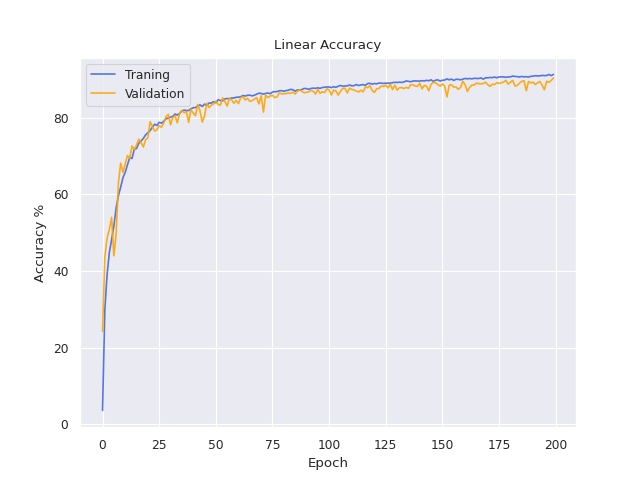
\includegraphics[width=.28\textwidth]{modelv0_linear_accuracy}}\hfill
  \subfloat{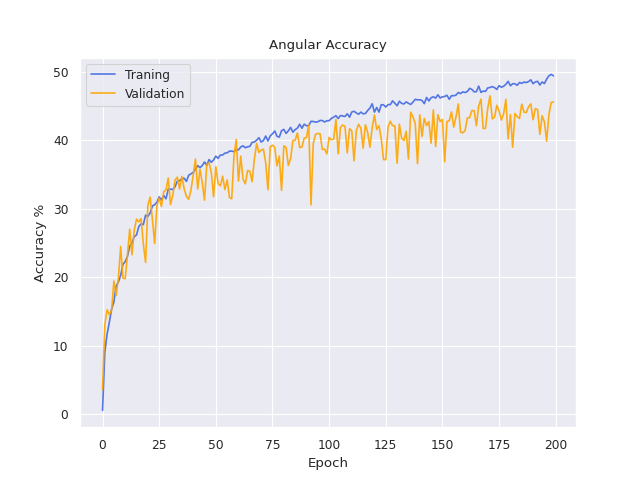
\includegraphics[width=.28\textwidth]{modelv0_angular_accuracy}}\hfill
  \subfloat{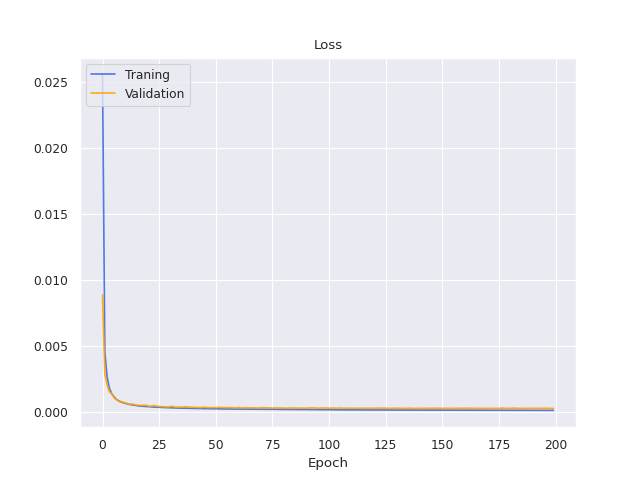
\includegraphics[width=.28\textwidth]{modelv0_loss}}\par
  \raisebox{35pt}{\parbox[b]{.1\textwidth}{modelv1}}%
  \subfloat{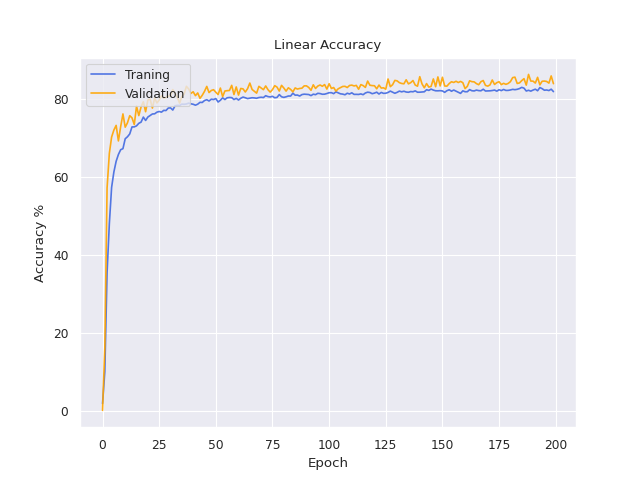
\includegraphics[width=.28\textwidth]{modelv1_linear_accuracy}}\hfill
  \subfloat{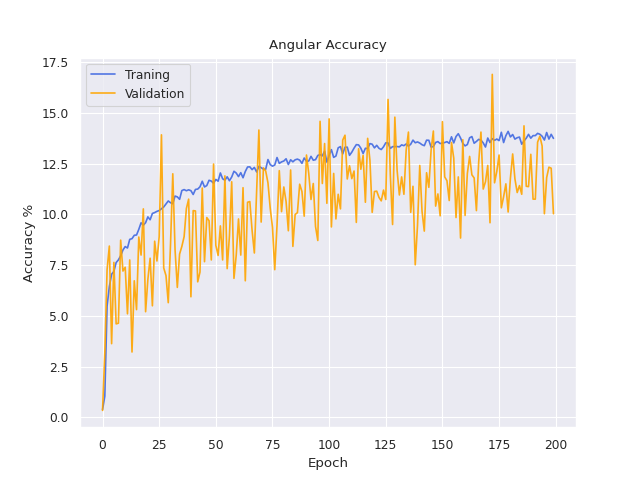
\includegraphics[width=.28\textwidth]{modelv1_angular_accuracy}}\hfill
  \subfloat{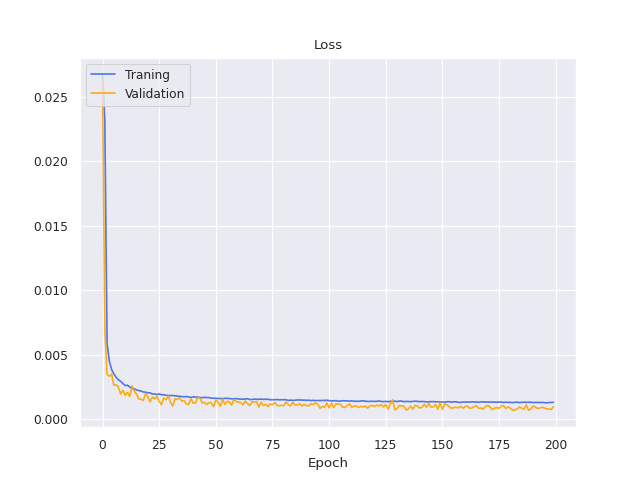
\includegraphics[width=.28\textwidth]{modelv1_loss}}
  \caption{Results from training the three different model architectures on dataset A, showing linear accuracy, angular accuracy, and loss achieved. A prediction was considered correct if the continuous velocity value was within 5\% of the label value.}
  \label{fig:training_results}
\end{figure}

\begin{figure}
  \centering
  \raisebox{35pt}{\parbox[b]{.1\textwidth}{modelv0}}%
  \subfloat{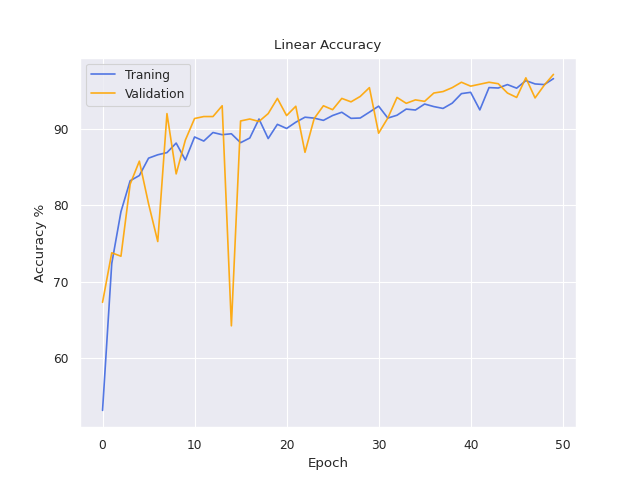
\includegraphics[width=.28\textwidth]{modelv0_200_fine_tuned_cw_ccw_linear_accuracy}}\hfill
  \subfloat{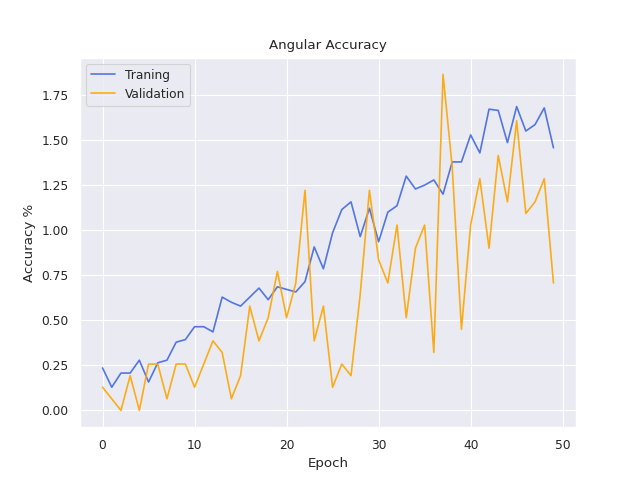
\includegraphics[width=.28\textwidth]{modelv0_200_fine_tuned_cw_ccw_angular_accuracy}}\hfill
  \subfloat{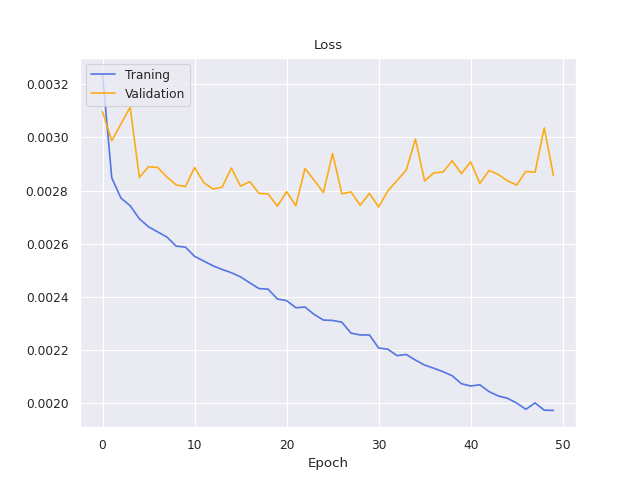
\includegraphics[width=.28\textwidth]{modelv0_200_fine_tuned_cw_ccw_loss}}\par
  \raisebox{35pt}{\parbox[b]{.1\textwidth}{modelv1}}%
  \subfloat{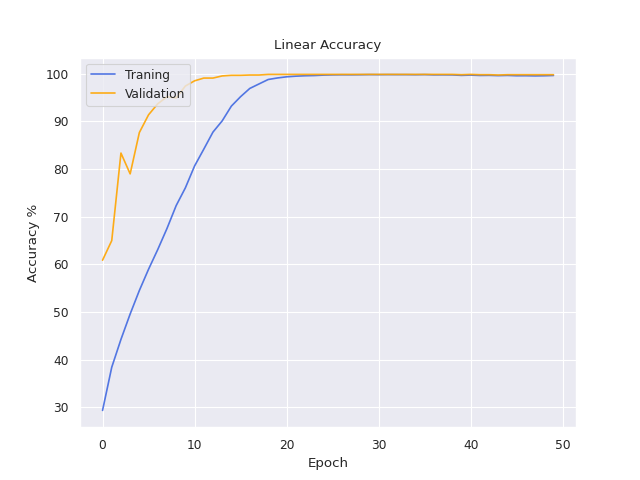
\includegraphics[width=.28\textwidth]{modelv1_200_fine_tuned_cw_ccw_linear_accuracy}}\hfill
  \subfloat{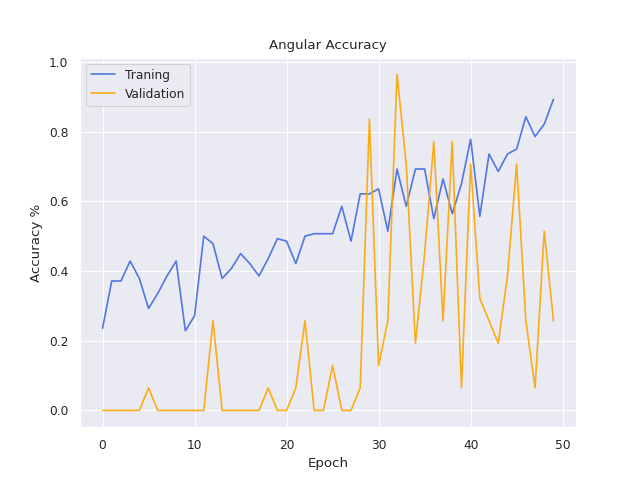
\includegraphics[width=.28\textwidth]{modelv1_200_fine_tuned_cw_ccw_angular_accuracy}}\hfill
  \subfloat{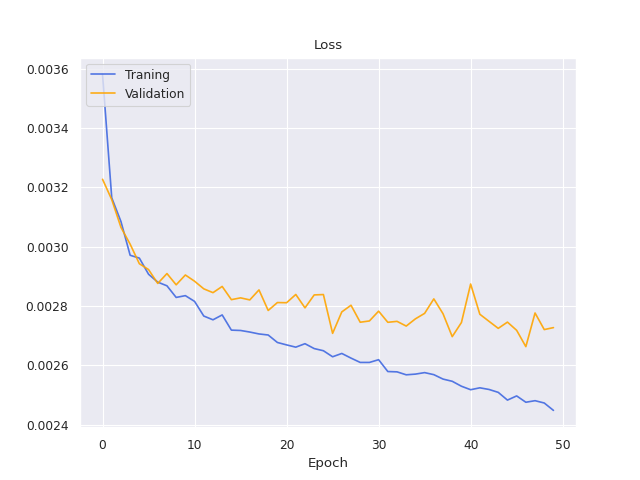
\includegraphics[width=.28\textwidth]{modelv1_200_fine_tuned_cw_ccw_loss}}\par
  \caption{Results from fine tuning the shared weights models on dataset B, showing linear accuracy, angular accuracy, and loss achieved. A prediction was considered correct if the continuous velocity value was within 5\% of the label value.}
  \label{fig:fine_tuning_training_results}
\end{figure}

\section{Performance Evaluations}

\subsection{Simulator and AIDO}

\todo 3x3 figure showing overview map trajectories from AIDO for initial 3 models on 3 maps
% \begin{figure}
%   \centering
%   \raisebox{35pt}{\parbox[b]{.1\textwidth}{nvidia}}%
%   \subfloat{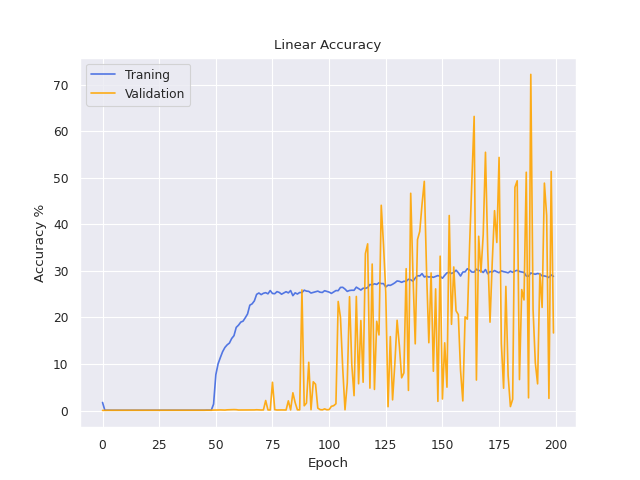
\includegraphics[width=.28\textwidth]{nvidia_linear_accuracy}}\hfill
%   \subfloat{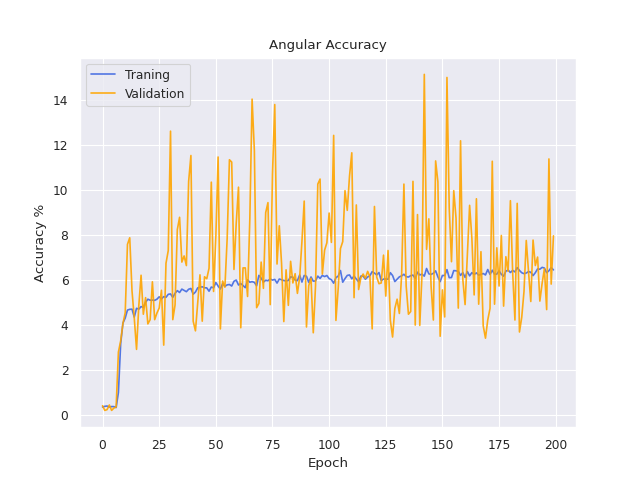
\includegraphics[width=.28\textwidth]{nvidia_angular_accuracy}}\hfill
%   \subfloat{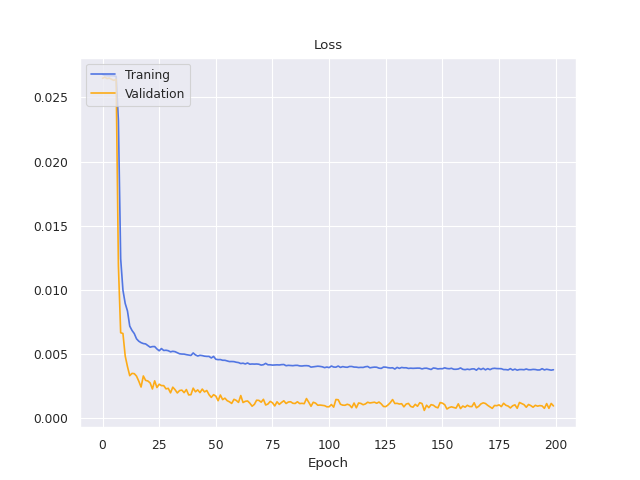
\includegraphics[width=.28\textwidth]{nvidia_loss}}\par
%   \raisebox{35pt}{\parbox[b]{.1\textwidth}{modelv0}}%
%   \subfloat{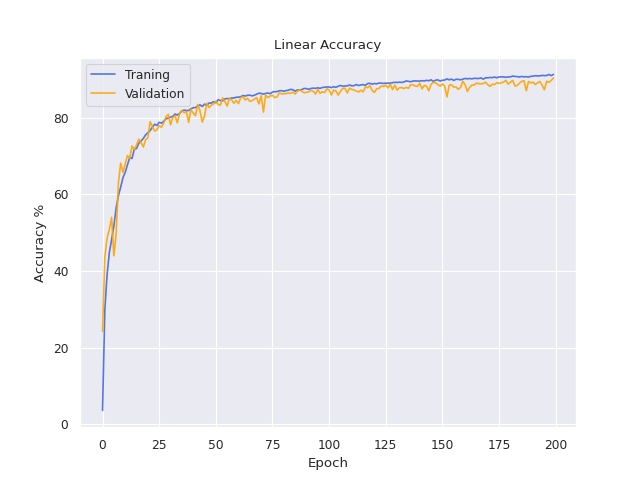
\includegraphics[width=.28\textwidth]{modelv0_linear_accuracy}}\hfill
%   \subfloat{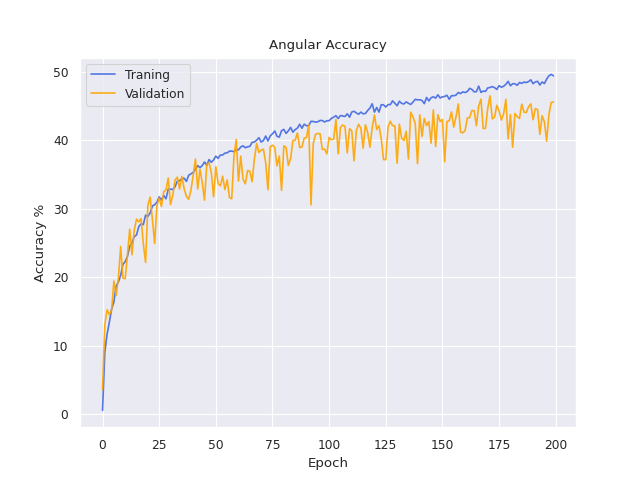
\includegraphics[width=.28\textwidth]{modelv0_angular_accuracy}}\hfill
%   \subfloat{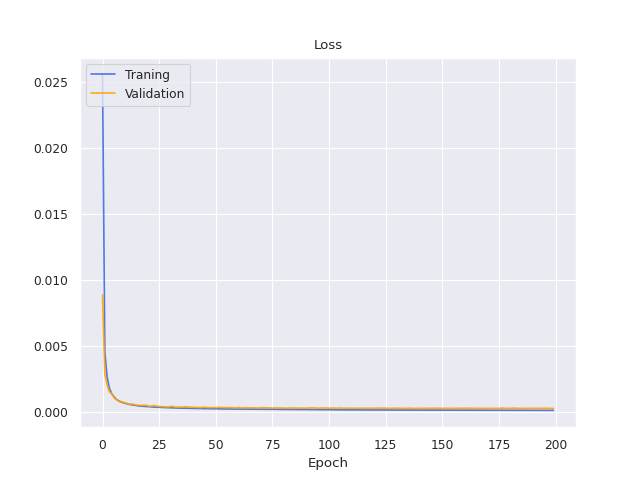
\includegraphics[width=.28\textwidth]{modelv0_loss}}\par
%   \raisebox{35pt}{\parbox[b]{.1\textwidth}{modelv1}}%
%   \subfloat{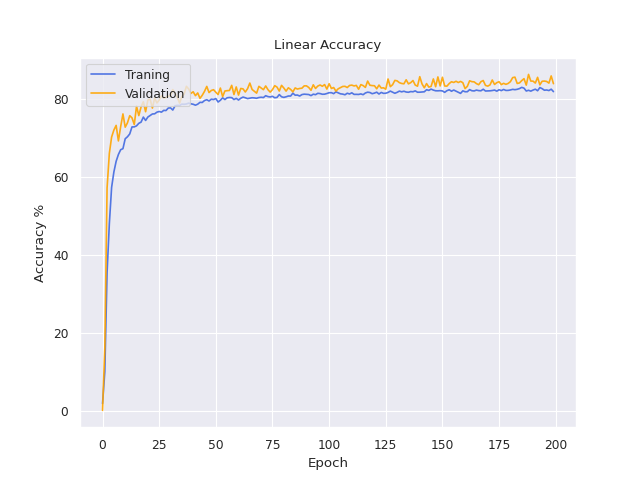
\includegraphics[width=.28\textwidth]{modelv1_linear_accuracy}}\hfill
%   \subfloat{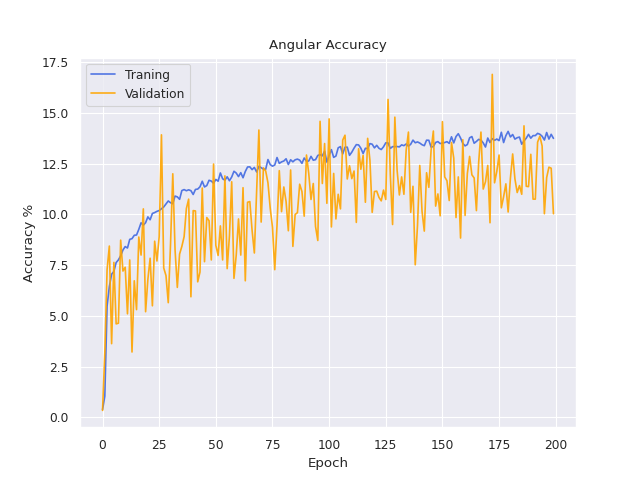
\includegraphics[width=.28\textwidth]{modelv1_angular_accuracy}}\hfill
%   \subfloat{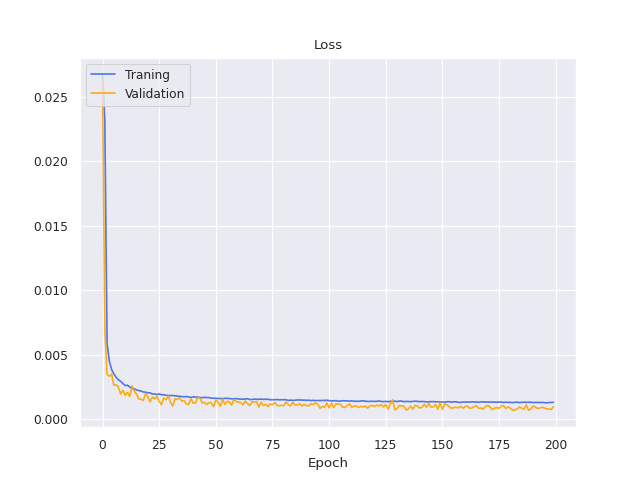
\includegraphics[width=.28\textwidth]{modelv1_loss}}
%   \caption{Results from training the three different model architectures on dataset A, showing linear accuracy, angular accuracy, and loss achieved. A prediction was considered correct if the continuous velocity value was within 5\% of the label value.}
%   \label{fig:training_results}
% \end{figure}

\todo 2x3 figure showing overview map trajectories from AIDO for modelv0+v1 with fine tuning on 3 maps

\todo Share links to videos from simulator and AIDO submissions

\todo Discuss quantative performance for each model including baseline

\subsection{Real World}

\todo Discuss quantative performance for each model including baseline

\todo Share links to videos for each map/model evaluated

Baselines map2:
\url{https://youtu.be/oNrlfTRxNy0}

Model v1 map2:
\url{https://youtu.be/NMiHz7VIw_4}

\section{Potential Future Improvements}

\todo Discuss algorithmic enhancements

\todo Discuss robot limitations

\bibliographystyle{alpha}
\bibliography{paper}

\end{document}
